\documentclass[a4paper,UTF8]{article}
\usepackage{ctex}
\usepackage[margin=1.25in]{geometry}
\usepackage{color}
\usepackage{graphicx}
\usepackage{amssymb}
\usepackage{amsmath}
\usepackage{amsthm}
\usepackage{enumerate}
\usepackage{bm}
\usepackage{hyperref}
\usepackage{epsfig}
\usepackage{color}
\usepackage{mdframed}
\usepackage{lipsum}
\usepackage{mathtools}
\usepackage{hyperref}
\usepackage{diagbox}
\usepackage{float}
\usepackage{caption}
\usepackage{algorithm}
\usepackage{algorithmicx}  
\usepackage{algpseudocode}
\usepackage{amsmath} 
\usepackage{graphicx}
\usepackage{subfigure}
\newmdtheoremenv{thm-box}{myThm}
\newmdtheoremenv{prop-box}{Proposition}
\newmdtheoremenv{def-box}{定义}
\usepackage{listings}
\usepackage{xcolor}
\lstset{
	numbers=left, 
	numberstyle= \tiny, 
	keywordstyle= \color{ blue!70},
	commentstyle= \color{red!50!green!50!blue!50}, 
	frame=shadowbox, % 阴影效果
	rulesepcolor= \color{ red!20!green!20!blue!20} ,
	escapeinside=``, % 英文分号中可写入中文
	xleftmargin=2em,xrightmargin=2em, aboveskip=1em,
	framexleftmargin=2em
} 

\usepackage{booktabs}

\setlength{\evensidemargin}{.25in}
\setlength{\textwidth}{6in}
\setlength{\topmargin}{-0.5in}
\setlength{\topmargin}{-0.5in}

% \setlength{\textheight}{9.5in}
%%%%%%%%%%%%%%%%%%此处用于设置页眉页脚%%%%%%%%%%%%%%%%%%
\usepackage{fancyhdr}                                
\usepackage{lastpage}                                           
\usepackage{layout}                                             
\footskip = 10pt 
\pagestyle{fancy}                    % 设置页眉                 
\lhead{研一下学期}                    
\chead{论文阅读笔记}                                                
% \rhead{第\thepage/\pageref{LastPage}页} 
\rhead{Step4}                                                                                               
\cfoot{\thepage}                                                
\renewcommand{\headrulewidth}{1pt}  			%页眉线宽,设为0可以去页眉线
\setlength{\skip\footins}{0.5cm}    			%脚注与正文的距离           
\renewcommand{\footrulewidth}{0pt}  			%页脚线宽,设为0可以去页脚线

\makeatletter 									%设置双线页眉                                        
\def\headrule{{\if@fancyplain\let\headrulewidth\plainheadrulewidth\fi%
\hrule\@height 1.0pt \@width\headwidth\vskip1pt	%上面线为1pt粗  
\hrule\@height 0.5pt\@width\headwidth  			%下面0.5pt粗            
\vskip-2\headrulewidth\vskip-1pt}      			%两条线的距离1pt        
 \vspace{6mm}}     								%双线与下面正文之间的垂直间距              
\makeatother  

%%%%%%%%%%%%%%%%%%%%%%%%%%%%%%%%%%%%%%%%%%%%%%
\numberwithin{equation}{section}
%\usepackage[thmmarks, amsmath, thref]{ntheorem}
\newtheorem{theorem}{Theorem}
\newtheorem*{definition}{Definition}
\newtheorem*{solution}{Solution}
\newtheorem*{prove}{Proof}
\newcommand{\indep}{\rotatebox[origin=c]{90}{$\models$}}

\usepackage{multirow}

%--

%--
\begin{document}
\title{论文阅读笔记\\
Step4}
\author{MF1833063, 史鹏, spwannasing@gmail.com}
\maketitle

\newpage
\section{Stochastic Answer Networks for Machine Reading Comprehension}

\newpage
\section{Multi-Granularity Hierarchical Attention Fusion Networks for Reading Comprehension and Question Answering}


\newpage
\section{A Multi-Stage Memory Augmented Neural Network for Machine Reading Comprehension}

\newpage
\section{S-NET: FROM ANSWER EXTRACTION TO ANSWER GENERATION FOR MACHINE READING COMPREHENSION}

\newpage
\section{QANET: COMBINING LOCAL CONVOLUTION WITH GLOBAL SELF-ATTENTION FOR READING COMPREHENSION}

\newpage
\section{Read + Verify: Machine Reading Comprehension with Unanswerable Questions}

\newpage
\section{Adversarial Examples for Evaluating Reading Comprehension Systems}

\newpage
\section{Reading Wikipedia to Answer Open-Domain Questions}
主要解决的是开放域问答,在这个论文里即:给出一个问题,从上万个wiki的document中找到答案,核心思想是分为两步,第一步document检索,找到和question最相关的几篇文章,然后第二步在这几篇document上运行常规的MRC算法即可。
我们的方法将基于bigram散列和tf-idf匹配的搜索组件与经过训练以检测维基百科段落中的答案的多层递归神经网络模型相结合。
\begin{figure}[H]
	\centering
	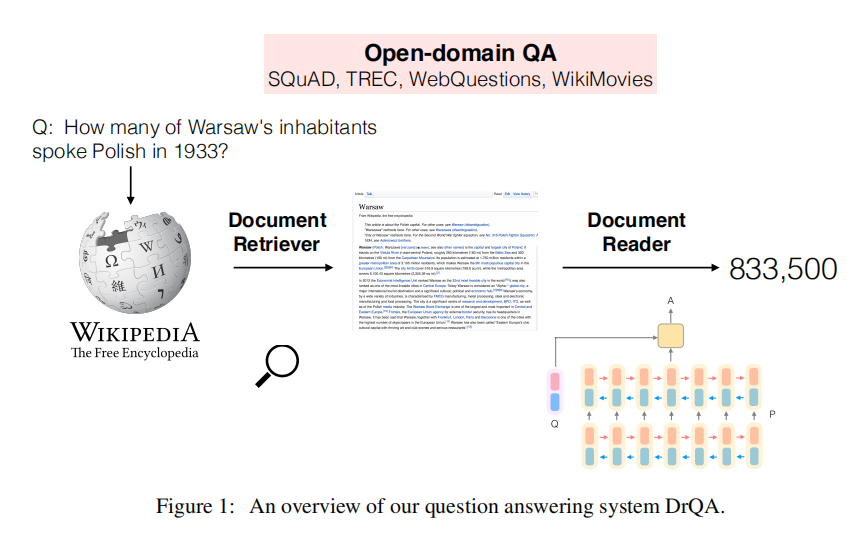
\includegraphics[width=\textwidth]{8-1.png}
\end{figure}
\newpage
\section{DRr-Net: Dynamic Re-read Network for Sentence Semantic Matching}
注意机制在捕捉语义关系和正确对齐两个句子的元素方面起着重要的作用。然而,句子在语义匹配过程中的重要部分随着句子理解程度的变化而动态变化。
因此提出了DRr-Net,每一步都要注意句子的一个小区域,重读重要的单词,以便更好地理解句子的语义。
重点是“Re”的思想,可以借鉴到MRC中。
\begin{figure}[H]
	\centering
	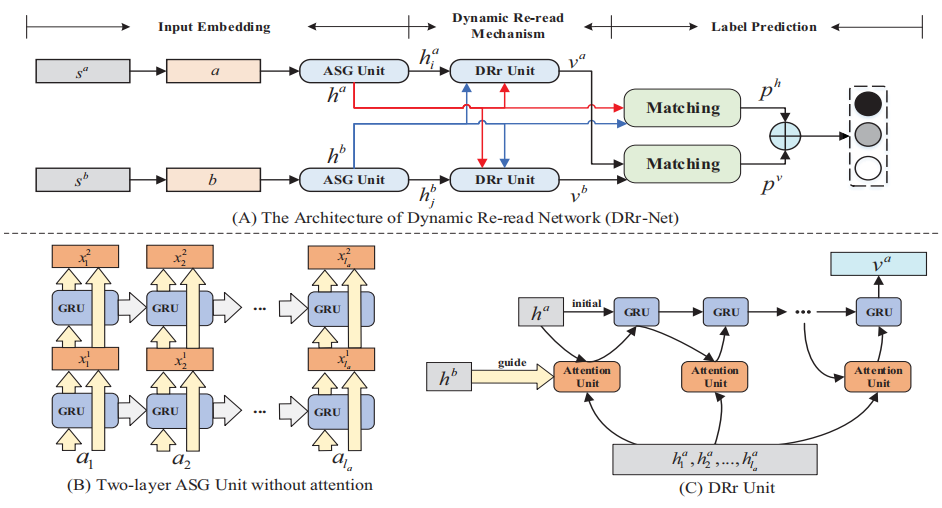
\includegraphics[width=\textwidth]{9-1.png}
\end{figure}

\newpage
\section{FLOWQA: GRASPING FLOW IN HISTORY FORCONVERSATIONAL MACHINE COMPREHENSION}
解决的问题的conversational阅读理解中对于之前的questions的记忆问题,通过“flow”来实现。核心思想是首先1个context对n个问题分别align,
然后经过contextual(bi-lstm)处理后,不同question对应的contex的同一位置的单词送入lstm,即每个lstm处理同一个单词对不同question 的align后的结果。
重复此操作三次。
\begin{figure}[H]
	\centering
	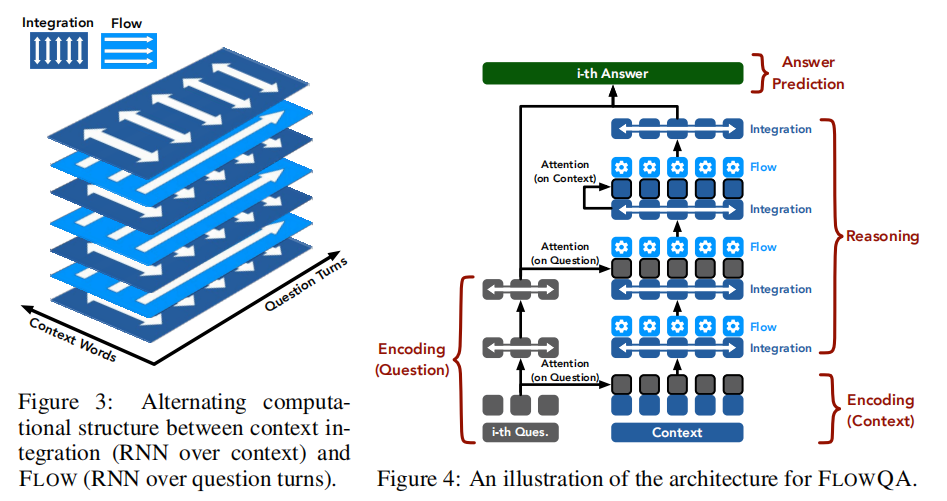
\includegraphics[width=\textwidth]{10-1.png}
\end{figure}
\begin{equation}
	\hat{C}_{i}^{h}=\hat{c}_{i, 1}^{h}, \ldots, \hat{c}_{i, m}^{h}=\operatorname{BiLSTM}\left(\left[\boldsymbol{C}_{i}^{h}\right]\right)
	\end{equation}
	\begin{equation}
		f_{1, j}^{h+1}, \ldots, f_{t, j}^{h+1}=\operatorname{GRU}\left(\hat{c}_{1, j}^{h}, \ldots, \hat{c}_{t, j}^{h}\right)
		\end{equation}
		\begin{equation}
		\begin{array}{c}{F_{i}^{h+1}=\left\{f_{i, 1}^{h+1}, \ldots, f_{i, m}^{h+1}\right\}} \\ {C_{i}^{h+1}=c_{i, 1}^{h+1}, \ldots, c_{i, m}^{h+1}=\left[\hat{c}_{i, 1}^{h} ; f_{i, 1}^{h+1}\right], \ldots,\left[\hat{c}_{i, m}^{h} ; f_{i, m}^{h+1}\right]}\end{array}
		\end{equation}
		\begin{equation}
			Q_{i}^{1}=q_{i, 1}^{1}, \ldots, q_{i, n}^{1}=\operatorname{BiLSTM}\left(Q_{i}\right), Q_{i}^{2}=q_{i, 1}^{2}, \ldots, q_{i, n}^{2}=\operatorname{BiLSTM}\left(Q_{i}^{1}\right)
			\end{equation}
			\begin{equation}
				\tilde{q}_{i}=\sum_{k=1}^{n} \alpha_{i, k} \cdot q_{i, k}^{2}, \alpha_{i, k} \propto \exp \left(w^{T} q_{i, k}^{2}\right)
				\end{equation}
				\begin{equation}
					p_{1}, \ldots, p_{t}=\operatorname{LSTM}\left(\tilde{q}_{i}, \ldots, \tilde{q}_{t}\right)
					\end{equation}
					\begin{equation}
					\begin{aligned} C_{i}^{1} &=\operatorname{IF}\left(C_{i}^{0}\right) \\ C_{i}^{2} &=\operatorname{IF}\left(C_{i}^{1}\right) \end{aligned}
					\end{equation}
					\begin{equation}
						\hat{q}_{i, j}=\sum_{k=1}^{n} \alpha^{i, j, k} \cdot q_{i, k}^{2}, \alpha^{i, j, k} \propto \exp \left(S\left(\left[c_{i} ; c_{j, i}^{1} ; c_{j, i}^{2}\right],\left[q_{j, k} ; q_{j, k}^{1} ; q_{j, k}^{2}\right]\right)\right)
						\end{equation}
						\begin{equation}
							C_{i}^{3}=\operatorname{IF}\left(\left[c_{i, 1}^{2} ; \hat{q}_{i, 1}\right], \ldots,\left[c_{i, m}^{2} ; \hat{q}_{i, m}\right]\right)
							\end{equation}
							\begin{equation}
								\hat{c}_{i, j}=\sum_{k=1}^{m} \alpha^{i, j, k} \cdot c_{i, k}^{3}, \alpha^{i, j, k} \propto \exp \left(S\left(\left[c_{i, j}^{1} ; c_{i, j}^{2}, c_{i, j}^{3}\right],\left[c_{i, k}^{1} ; c_{i, k}^{2}, c_{i, k}^{3}\right]\right)\right)
								\end{equation}
								\begin{equation}
									C_{i}^{4}=\operatorname{BiLSTM}\left(\left[c_{i, 1}^{3} ; \hat{c}_{i, 1}\right], \ldots,\left[c_{i, m}^{3} ; \hat{c}_{i, m}\right]\right)
									\end{equation}
\end{document}